\appendix
\section*{APPENDIX}

\section{Augmented Results}


In this section, we provide additional information to augment results provided in our time series case study. 
Table~\ref{tab:sample} displays the proportion of data required to attain a given $TLB$ when using a PCA transformation where output dimension is equal to input dimension. Table~\ref{tab:kneeded} illustrates the output dimension required for each algorithm (PAA, FFT, and PCA) to attain a target $TLB$. 
Table~\ref{tab:runtime-comparison} illustrates the different running times of each algorithm (PAA, FFT, and PCA), and how sampling using the proportion from Table~\ref{tab:sample} for $TLB=0.99$ can help bridge the time gap between SVD and other techniques. 
%Finally, we provide all of the remaining lesion studies for the UCR dataset.


\begin{table}[]
\centering
\caption{Normalized lower dimension for target $TLB$ across DR techniques. PCA admits lower dimension for most UCR time series datasets.}
\label{tab:kneeded}
\scriptsize
\begin{tabular}{|l|r|r|r|r|r|r|}
\hline
                                  & \multicolumn{3}{c|}{\textbf{TLB:0.75}}     & \multicolumn{3}{c|}{\textbf{TLB:0.99}}     \\ \hline
\textbf{Dataset (dimension)} & \textit{PAA} & \textit{FFT} & \textit{PCA} & \textit{PAA} & \textit{FFT} & \textit{PCA} \\ \hline
ElectricDevices (96)              & 0.126        & 0.094        & 0.032        & 0.594        & 0.212        & 0.164        \\ \hline
FordA (500)                       & 0.138        & 0.098        & 0.038        & 0.636        & 0.214        & 0.17         \\ \hline
FordB (500)                       & 0.018        & 0.029        & 0.009        & 0.290        & 0.177        & 0.035        \\ \hline
MALLAT (1024)                     & 0.084        & 0.068        & 0.057        & 0.898        & 0.837        & 0.522        \\ \hline
Phoneme (1024)                    & 0.004        & 0.026        & 0.001        & 0.049        & 0.035        & 0.034        \\ \hline
StarLightCurves (1024)            & 0.015        & 0.028        & 0.019        & 0.037        & 0.086        & 0.062        \\ \hline
UWGLAll (945)                     & 0.078        & 0.065        & 0.026        & 0.822        & 0.736        & 0.322        \\ \hline
wafer (152)                       & 0.014        & 0.030        & 0.007        & 0.103        & 0.049        & 0.037        \\ \hline
yoga (426)                        & 0.375        & 0.375        & 0.281        & 0.812        & 0.822        & 0.770        \\ \hline

\end{tabular}
\end{table}



\begin{table}[]
\centering
\caption{Runtime (in ms) of 3 DR techniques. PCA is slowest, and can be over $56\times$ slower than PAA. Running SVD over a sample can bridge this gap.}
\label{tab:runtime-comparison}
\scriptsize
\begin{tabular}{|l|c|c|c|c|}
\hline
\textbf{Dataset}        & \textbf{PAA ($\times$SVD)} & \textbf{FFT} & \textbf{SVD} & \textbf{Sampling} \\ \hline
ElectricDevices         & 3 (9.8$\times$)            & 18           & 33           & 6                 \\ \hline
FordA                   & 7 (19$\times$)             & 38           & 137          & 8                 \\ \hline
FordB                   & 7 (18$\times$)             & 32           & 121          & 7                 \\ \hline
MALLAT                  & 7 (37.6$\times$)           & 35           & 278          & 5                 \\ \hline
Phoneme                 & 5 (56.2$\times$)           & 29           & 281          & 164               \\ \hline
StarLightCurves         & 19 (24.1$\times$)          & 120          & 457          & 5                 \\ \hline
UWGLAll & 7 (43.5$\times$)           & 56           & 287          & 8                 \\ \hline
Wafer                   & 4 (6.1$\times$)            & 13           & 22           & 5                 \\ \hline
Yoga                    & 4 (21.2$\times$)           & 29           & 81           & 8                 \\ \hline
\end{tabular}
\end{table}



\begin{table}[]
\centering
\scriptsize
\caption{A small proportion of data is needed to obtain a $TLB$-preserving transform with full PCA (output = input dimension).}

\begin{tabular}{|l|r|r|r|}
\hline
                               & \multicolumn{3}{c|}{\textit{\textbf{TLB}}}    \\ \hline
\textbf{Dataset (number of datapoints)}               & \textbf{0.75} & \textbf{0.90} & \textbf{0.99} \\ \hline
ElectricDevices (16637)               & 0.0026        & 0.0043        & 0.0088        \\ \hline
FordA   (4921)                       & 0.0054        & 0.0114        & 0.0198        \\ \hline
FordB   (4446)                       & 0.008         & 0.0146        & 0.0248        \\ \hline
MALLAT  (2400)                       & 0.0031        & 0.009         & 0.0197        \\ \hline
Phoneme   (2110)                     & 0.0547        & 0.1346        & 0.3875        \\ \hline
StarLightCurves (9236)               & 0.001         & 0.0011        & 0.0039        \\ \hline
UWGLAll  (4478)       & 0.0025        & 0.0056        & 0.024         \\ \hline
wafer  (7164)                        & 0.001         & 0.0032        & 0.0097        \\ \hline
yoga  (3300)                         & 0.0017        & 0.0028        & 0.0096        \\ \hline
\end{tabular}
\label{tab:sample}
\end{table}






\begin{comment}
\begin{table}[b]
\centering
\scriptsize
\caption{End-to-End runtime comparison of DROP and baseline techniques with k-NN retrieval task, in ms}
\label{tab:eefull}
\begin{tabular}{|l|c|c|c|c|c|}
\hline
\textbf{Dataset}       & \textbf{No DR} & \textbf{SVD} & \textbf{SVD-Halko} & \textbf{Oracle} & \textbf{DROP} \\ \hline
ChlorineConcentration  & 458   & 4054  & 424   & 207   & 178   \\ \hline
CinC                   & 1809  & 3068  & 5738  & 884   & 894   \\ \hline
ECG5000                & 1855  & 5689  & 561   & 362   & 482   \\ \hline
ElectricDevices        & 38222 & 83302 & 28433 & 27260 & 30701 \\ \hline
FordA                  & 21906 & 10546 & 5300  & 4270  & 4286  \\ \hline
FordB                  & 18271 & 8984  & 4917  & 3773  & 3792  \\ \hline
HandOutlines           & 5160  & 5620  & 9479  & 2832  & 2678  \\ \hline
InlineSkate            & 579   & 1420  & 2081  & 548   & 704   \\ \hline
InsectWingbeatSound    & 805   & 977   & 425   & 200   & 212   \\ \hline
MALLAT                 & 2593  & 2895  & 3870  & 643   & 450   \\ \hline
NonInvasiveFatalECG    & 5157  & 5229  & 3235  & 944   & 1043  \\ \hline
Phoneme                & 8490  & 6710  & 7687  & 7534  & 10446 \\ \hline
StarLightCurves        & 32024 & 35129 & 11429 & 1079  & 1238  \\ \hline
Two                    & 5728  & 8916  & 2849  & 2860  & 3335  \\ \hline
UWaveGestureLibraryAll & 25825 & 8147  & 5509  & 1298  & 1355  \\ \hline
uWaveGestureLibrary    & 4734  & 5669  & 1067  & 402   & 310   \\ \hline
wafer                  & 1536  & 12911 & 749   & 403   & 403   \\ \hline
yoga                   & 1199  & 2943  & 1029  & 174   & 153   \\ \hline
\end{tabular}
\end{table}


\begin{table}[b]
\centering
\scriptsize
\caption{Raw accuracy in k-NN retrieval task}
\label{tab:knn}
\begin{tabular}{|l|c|c|c|c|}
\hline
\textbf{Dataset}   & \textbf{SVD} & \textbf{SVD-Halko} & \textbf{Oracle} & \textbf{DROP} \\ \hline
ChlorineConcentration  & 0.893        & 0.886              & 0.906           & 0.903         \\ \hline
CinC                   & 0.894        & 0.892              & 0.899           & 0.929         \\ \hline
ECG5000                & 0.855        & 0.855              & 0.856           & 0.874         \\ \hline
ElectricDevices        & 0.877        & 0.875              & 0.866           & 0.888         \\ \hline
FordA                  & 0.892        & 0.878              & 0.884           & 0.9           \\ \hline
FordB                  & 0.875        & 0.875              & 0.871           & 0.874         \\ \hline
HandOutlines           & 0.908        & 0.901              & 0.907           & 0.92          \\ \hline
InlineSkate            & 0.832        & 0.818              & 0.803           & 0.805         \\ \hline
InsectWingbeatSound    & 0.815        & 0.815              & 0.811           & 0.848         \\ \hline
MALLAT                 & 0.83         & 0.83               & 0.876           & 0.892         \\ \hline
NonInvasiveFatalECG    & 0.82         & 0.822              & 0.836           & 0.827         \\ \hline
Phoneme                & 0.848        & 0.852              & 0.68            & 0.678         \\ \hline
StarLightCurves        & 0.615        & 0.648              & 0.653           & 0.651         \\ \hline
Two                    & 0.899        & 0.903              & 0.901           & 0.902         \\ \hline
UWaveGestureLibraryAll & 0.846        & 0.853              & 0.856           & 0.883         \\ \hline
uWaveGestureLibrary    & 0.797        & 0.797              & 0.808           & 0.838         \\ \hline
wafer                  & 0.808        & 0.818              & 0.833           & 0.888         \\ \hline
yoga                   & 0.791        & 0.791              & 0.797           & 0.818         \\ \hline
\end{tabular}
\end{table}


\end{comment}


\begin{comment}
\begin{table*}[]
\centering
\scriptsize
\caption{Output dimension required for target $TLB$ across dimensionality reduction technique (right 9 data columns), and proportion of data required to obtain a $TLB$-preserving PCA transformation with output dimension = input dimension (final 3 columns)}
\label{tab:bigtab}
\begin{tabular}{| c ||ccc|ccc|ccc||cc||ccc|}
\hline

 & \multicolumn{3}{c|}{\textbf{TLB: 0.75}} & \multicolumn{3}{c|}{\textbf{TLB: 0.90}} & \multicolumn{3}{c||}{\textbf{TLB: 0.99}} &  &  & \multicolumn{3}{c|}{\textbf{TLB}}  \\

\textbf{Dataset} & \textit{PAA }     & \textit{FFT}     & \textit{PCA}     & \textit{PAA}      & \textit{FFT}      & \textit{PCA}     & \textit{PAA}      & \textit{FFT}     &\textit{PCA}     &  &  & \textit{0.75}   & \textit{0.90 }  & \textit{0.99}   \\
\hline
50words                        & 9        & 9        & 7       & 18       & 14       & 10      & 62       & 28       & 25      &  &  & 0.0106 & 0.0185 & 0.0391 \\
Adiac                          & 7        & 8        & 4       & 15       & 13       & 6       & 69       & 34       & 20      &  &  & 0.0077 & 0.0145 & 0.0484 \\
ArrowHead                      & 9        & 9        & 4       & 16       & 13       & 8       & 73       & 33       & 26      &  &  & 0.0285 & 0.0626 & 0.2907 \\
Beef                           & 7        & 15       & 2       & 20       & 18       & 3       & 89       & 48       & 7       &  &  & 0.0494 & 0.0898 & 0.19   \\
BeetleFly                      & 16       & 16       & 6       & 28       & 21       & 12      & 99       & 34       & 22      &  &  & 0.3073 & 0.4449 & 0.7979 \\
BirdChicken                    & 8        & 14       & 3       & 14       & 17       & 6       & 48       & 20       & 15      &  &  & 0.156  & 0.2357 & 0.5437 \\
Car                            & 7        & 16       & 2       & 15       & 19       & 6       & 70       & 37       & 24      &  &  & 0.0428 & 0.0979 & 0.3719 \\
CBF                            & 15       & 13       & 7       & 61       & 57       & 45      & 114      & 114      & 107     &  &  & 0.0273 & 0.0775 & 0.1407 \\
ChlorineConcentration          & 46       & 34       & 2       & 93       & 81       & 5       & 153      & 153      & 30      &  &  & 0.001  & 0.0029 & 0.014  \\
CinC                           & 29       & 44       & 26      & 58       & 53       & 40      & 241      & 107      & 48      &  &  & 0.007  & 0.0157 & 0.0391 \\
Coffee                         & 14       & 17       & 3       & 46       & 37       & 6       & 225      & 158      & 38      &  &  & 0.1224 & 0.2715 & 0.8632 \\
Computers                      & 21       & 24       & 16      & 94       & 66       & 44      & 636      & 614      & 192     &  &  & 0.0596 & 0.1889 & 0.6818 \\
Cricket                        & 14       & 14       & 9       & 47       & 35       & 21      & 248      & 202      & 113     &  &  & 0.0198 & 0.0574 & 0.2488 \\
DiatomSizeReduction            & 7        & 11       & 7       & 11       & 13       & 10      & 87       & 55       & 21      &  &  & 0.015  & 0.0282 & 0.176  \\
DistalPhalanxOutlineAgeGroup   & 12       & 12       & 2       & 27       & 17       & 6       & 66       & 60       & 36      &  &  & 0.0094 & 0.0241 & 0.0987 \\
DistalPhalanxOutlineCorrect    & 12       & 12       & 2       & 26       & 16       & 7       & 66       & 57       & 32      &  &  & 0.006  & 0.0168 & 0.0642 \\
DistalPhalanxTW                & 12       & 12       & 2       & 27       & 16       & 6       & 66       & 60       & 34      &  &  & 0.0097 & 0.0236 & 0.098  \\
Earthquakes                    & 276      & 269      & 103     & 410      & 400      & 190     & 491      & 490      & 340     &  &  & 0.3733 & 0.6052 & 0.8988 \\
ECG200                         & 8        & 7        & 3       & 29       & 22       & 6       & 72       & 56       & 41      &  &  & 0.0288 & 0.0942 & 0.3287 \\
ECG5000                        & 14       & 14       & 3       & 30       & 24       & 7       & 115      & 88       & 31      &  &  & 0.001  & 0.0025 & 0.0132 \\
ECGFiveDays                    & 31       & 28       & 2       & 53       & 40       & 5       & 111      & 65       & 13      &  &  & 0.0073 & 0.0114 & 0.0275 \\
ElectricDevices                & 36       & 36       & 27      & 62       & 57       & 49      & 78       & 79       & 74      &  &  & 0.0026 & 0.0043 & 0.0088 \\
FaceAll                        & 28       & 24       & 8       & 50       & 35       & 20      & 110      & 81       & 48      &  &  & 0.0078 & 0.0171 & 0.0355 \\
FaceFour                       & 36       & 31       & 5       & 67       & 43       & 12      & 277      & 228      & 61      &  &  & 0.1143 & 0.2727 & 0.7708 \\
FacesUCR                       & 28       & 24       & 9       & 48       & 34       & 22      & 109      & 53       & 49      &  &  & 0.0077 & 0.0169 & 0.0355 \\
FISH                           & 10       & 15       & 5       & 20       & 18       & 11      & 91       & 37       & 28      &  &  & 0.0181 & 0.0433 & 0.1587 \\
FordA                          & 63       & 47       & 16      & 98       & 61       & 35      & 297      & 106      & 82      &  &  & 0.0054 & 0.0114 & 0.0198 \\
FordB                          & 69       & 49       & 19      & 102      & 65       & 39      & 318      & 107      & 85      &  &  & 0.008  & 0.0146 & 0.0248 \\
Gun                            & 5        & 6        & 3       & 11       & 9        & 5       & 56       & 24       & 14      &  &  & 0.0282 & 0.0477 & 0.134  \\
Ham                            & 34       & 32       & 7       & 73       & 58       & 18      & 261      & 114      & 61      &  &  & 0.0811 & 0.1558 & 0.4486 \\
HandOutlines                   & 11       & 70       & 10      & 25       & 83       & 32      & 93       & 91       & 46      &  &  & 0.0045 & 0.0091 & 0.0372 \\
Haptics                        & 10       & 29       & 6       & 19       & 35       & 14      & 173      & 81       & 32      &  &  & 0.017  & 0.0394 & 0.1234 \\
Herring                        & 10       & 15       & 3       & 25       & 18       & 8       & 111      & 63       & 39      &  &  & 0.0599 & 0.1447 & 0.4878 \\
InlineSkate                    & 7        & 49       & 7       & 15       & 58       & 17      & 55       & 63       & 22      &  &  & 0.0085 & 0.0162 & 0.0388 \\
InsectWingbeatSound            & 15       & 14       & 7       & 28       & 22       & 13      & 100      & 42       & 33      &  &  & 0.0048 & 0.0119 & 0.0255 \\
ItalyPowerDemand               & 6        & 6        & 2       & 11       & 10       & 5       & 19       & 17       & 15      &  &  & 0.0068 & 0.01   & 0.0198 \\
LargeKitchenAppliances         & 59       & 49       & 36      & 165      & 125      & 89      & 624      & 545      & 284     &  &  & 0.0987 & 0.2373 & 0.6068 \\
Lighting2                      & 41       & 34       & 9       & 152      & 149      & 28      & 557      & 490      & 82      &  &  & 0.186  & 0.4505 & 0.9132 \\
Lighting7                      & 31       & 27       & 9       & 126      & 118      & 26      & 280      & 269      & 81      &  &  & 0.1439 & 0.3534 & 0.9022 \\
MALLAT                         & 19       & 30       & 10      & 46       & 36       & 26      & 297      & 182      & 36      &  &  & 0.0031 & 0.009  & 0.0197 \\
Meat                           & 13       & 14       & 2       & 32       & 24       & 4       & 218      & 213      & 23      &  &  & 0.0398 & 0.0528 & 0.3494 \\
MedicalImages                  & 12       & 10       & 3       & 20       & 17       & 7       & 66       & 34       & 17      &  &  & 0.007  & 0.0103 & 0.0256 \\
MiddlePhalanxOutlineAgeGroup   & 12       & 12       & 2       & 27       & 16       & 4       & 66       & 60       & 31      &  &  & 0.0096 & 0.0191 & 0.0939 \\
MiddlePhalanxOutlineCorrect    & 12       & 12       & 2       & 27       & 16       & 5       & 66       & 58       & 30      &  &  & 0.0065 & 0.0127 & 0.0548 \\
MiddlePhalanxTW                & 12       & 12       & 2       & 27       & 16       & 5       & 66       & 60       & 32      &  &  & 0.0089 & 0.0206 & 0.0916 \\
MoteStrain                     & 12       & 11       & 7       & 39       & 37       & 26      & 76       & 75       & 63      &  &  & 0.0148 & 0.0323 & 0.0838 \\
NonInvasiveFatalECG            & 16       & 22       & 3       & 42       & 31       & 18      & 201      & 121      & 82      &  &  & 0.0021 & 0.0043 & 0.0375 \\
OliveOil                       & 33       & 25       & 2       & 61       & 51       & 5       & 375      & 213      & 23      &  &  & 0.0936 & 0.1727 & 0.6366 \\
OSULeaf                        & 11       & 13       & 9       & 20       & 16       & 14      & 73       & 30       & 29      &  &  & 0.0258 & 0.0435 & 0.1104 \\
PhalangesOutlinesCorrect       & 11       & 12       & 2       & 26       & 16       & 5       & 65       & 56       & 28      &  &  & 0.0023 & 0.0046 & 0.0187 \\
Phoneme                        & 87       & 70       & 59      & 268      & 201      & 160     & 920      & 858      & 535     &  &  & 0.0547 & 0.1346 & 0.3875 \\
Plane                          & 12       & 11       & 3       & 22       & 14       & 6       & 76       & 39       & 21      &  &  & 0.0285 & 0.0683 & 0.2068 \\
ProximalPhalanxOutlineAgeGroup & 12       & 12       & 2       & 26       & 18       & 4       & 65       & 58       & 28      &  &  & 0.0068 & 0.0171 & 0.0825 \\
ProximalPhalanxOutlineCorrect  & 12       & 12       & 2       & 27       & 18       & 5       & 66       & 58       & 28      &  &  & 0.0046 & 0.0134 & 0.0512 \\
ProximalPhalanxTW              & 12       & 12       & 2       & 26       & 18       & 5       & 65       & 59       & 28      &  &  & 0.0052 & 0.0153 & 0.0831 \\
RefrigerationDevices           & 94       & 76       & 60      & 222      & 154      & 121     & 645      & 586      & 316     &  &  & 0.1414 & 0.2777 & 0.6696 \\
ScreenType                     & 18       & 24       & 20      & 70       & 55       & 40      & 614      & 614      & 207     &  &  & 0.0324 & 0.1087 & 0.5341 \\
ShapeletSim                    & 275      & 272      & 62      & 410      & 402      & 111     & 491      & 490      & 180     &  &  & 0.497  & 0.7498 & 0.969  \\
ShapesAll                      & 7        & 14       & 7       & 14       & 17       & 14      & 49       & 25       & 20      &  &  & 0.0048 & 0.0137 & 0.0278 \\
SmallKitchenAppliances         & 259      & 235      & 104     & 497      & 423      & 204     & 698      & 678      & 398     &  &  & 0.2489 & 0.422  & 0.7194 \\
SonyAIBORobotSurface           & 15       & 14       & 5       & 28       & 21       & 13      & 56       & 43       & 38      &  &  & 0.0211 & 0.0442 & 0.0969 \\
SonyAIBORobotSurfaceII         & 18       & 18       & 6       & 30       & 24       & 13      & 57       & 45       & 39      &  &  & 0.0143 & 0.0272 & 0.0708 \\
StarLightCurves                & 5        & 27       & 2       & 14       & 33       & 21      & 51       & 36       & 35      &  &  & 0.001  & 0.0011 & 0.0039 \\
Strawberry                     & 10       & 11       & 2       & 24       & 21       & 6       & 98       & 41       & 13      &  &  & 0.005  & 0.0086 & 0.0225 \\
SwedishLeaf                    & 9        & 9        & 5       & 19       & 14       & 10      & 71       & 37       & 32      &  &  & 0.0083 & 0.0178 & 0.0727 \\
Symbols                        & 7        & 11       & 6       & 12       & 13       & 11      & 46       & 26       & 14      &  &  & 0.0071 & 0.0096 & 0.0246 \\
synthetic                      & 14       & 14       & 7       & 37       & 38       & 28      & 58       & 59       & 54      &  &  & 0.0281 & 0.0642 & 0.0964 \\
ToeSegmentation1               & 12       & 10       & 8       & 24       & 19       & 16      & 116      & 49       & 43      &  &  & 0.0548 & 0.0992 & 0.2988 \\
ToeSegmentation2               & 10       & 13       & 6       & 21       & 20       & 13      & 101      & 49       & 34      &  &  & 0.0718 & 0.144  & 0.3784 \\
Trace                          & 6        & 9        & 2       & 18       & 17       & 7       & 120      & 69       & 31      &  &  & 0.0222 & 0.0555 & 0.3752 \\
TwoLeadECG                     & 12       & 9        & 2       & 25       & 19       & 4       & 70       & 51       & 14      &  &  & 0.0045 & 0.0081 & 0.0259 \\
Two                            & 13       & 11       & 7       & 34       & 24       & 20      & 108      & 102      & 98      &  &  & 0.0038 & 0.0097 & 0.0259 \\
UWaveGestureLibraryAll         & 15       & 27       & 18      & 35       & 32       & 28      & 151      & 82       & 59      &  &  & 0.0025 & 0.0056 & 0.024  \\
uWaveGestureLibrary            & 4        & 10       & 5       & 10       & 11       & 10      & 43       & 27       & 20      &  &  & 0.0017 & 0.0024 & 0.0081 \\
wafer                          & 12       & 10       & 4       & 37       & 29       & 11      & 125      & 112      & 49      &  &  & 0.001  & 0.0032 & 0.0097 \\
Wine                           & 10       & 9        & 2       & 27       & 20       & 3       & 104      & 58       & 9       &  &  & 0.031  & 0.0477 & 0.1745 \\
WordsSynonyms                  & 9        & 9        & 7       & 17       & 14       & 10      & 62       & 31       & 25      &  &  & 0.0094 & 0.0196 & 0.0389 \\
Worms                          & 9        & 26       & 8       & 26       & 30       & 17      & 123      & 62       & 41      &  &  & 0.0661 & 0.109  & 0.3177 \\
WormsTwoClass                  & 10       & 26       & 8       & 25       & 30       & 17      & 124      & 61       & 42      &  &  & 0.0575 & 0.1193 & 0.3289 \\
yoga                           & 6        & 13       & 3       & 11       & 15       & 11      & 44       & 21       & 16      &  &  & 0.0017 & 0.0028 & 0.0096 \\
\hline
\end{tabular}
\end{table*}
\end{comment}


\begin{comment}
\begin{table}[H]
\centering
\scriptsize
\caption{Proportion of data required to obtain a $TLB$-preserving transformation with full PCA (i.e., output dimension = input dimension)}

\begin{tabular}{|l|c|c|c|}
\hline
                               & \multicolumn{3}{c|}{\textit{\textbf{TLB}}}    \\ \hline
\textbf{Dataset}               & \textbf{0.75} & \textbf{0.90} & \textbf{0.99} \\ \hline
50words                        & 0.0106        & 0.0185        & 0.0391        \\ \hline
Adiac                          & 0.0077        & 0.0145        & 0.0484        \\ \hline
ArrowHead                      & 0.0285        & 0.0626        & 0.2907        \\ \hline
Beef                           & 0.0494        & 0.0898        & 0.19          \\ \hline
BeetleFly                      & 0.3073        & 0.4449        & 0.7979        \\ \hline
BirdChicken                    & 0.156         & 0.2357        & 0.5437        \\ \hline
Car                            & 0.0428        & 0.0979        & 0.3719        \\ \hline
CBF                            & 0.0273        & 0.0775        & 0.1407        \\ \hline
ChlorineConcentration          & 0.001         & 0.0029        & 0.014         \\ \hline
CinC                           & 0.007         & 0.0157        & 0.0391        \\ \hline
Coffee                         & 0.1224        & 0.2715        & 0.8632        \\ \hline
Computers                      & 0.0596        & 0.1889        & 0.6818        \\ \hline
Cricket                        & 0.0198        & 0.0574        & 0.2488        \\ \hline
DiatomSizeReduction            & 0.015         & 0.0282        & 0.176         \\ \hline
DistalPhalanxOutlineAgeGroup   & 0.0094        & 0.0241        & 0.0987        \\ \hline
DistalPhalanxOutlineCorrect    & 0.006         & 0.0168        & 0.0642        \\ \hline
DistalPhalanxTW                & 0.0097        & 0.0236        & 0.098         \\ \hline
Earthquakes                    & 0.3733        & 0.6052        & 0.8988        \\ \hline
ECG200                         & 0.0288        & 0.0942        & 0.3287        \\ \hline
ECG5000                        & 0.001         & 0.0025        & 0.0132        \\ \hline
ECGFiveDays                    & 0.0073        & 0.0114        & 0.0275        \\ \hline
ElectricDevices                & 0.0026        & 0.0043        & 0.0088        \\ \hline
FaceAll                        & 0.0078        & 0.0171        & 0.0355        \\ \hline
FaceFour                       & 0.1143        & 0.2727        & 0.7708        \\ \hline
FacesUCR                       & 0.0077        & 0.0169        & 0.0355        \\ \hline
FISH                           & 0.0181        & 0.0433        & 0.1587        \\ \hline
FordA                          & 0.0054        & 0.0114        & 0.0198        \\ \hline
FordB                          & 0.008         & 0.0146        & 0.0248        \\ \hline
Gun                            & 0.0282        & 0.0477        & 0.134         \\ \hline
Ham                            & 0.0811        & 0.1558        & 0.4486        \\ \hline
HandOutlines                   & 0.0045        & 0.0091        & 0.0372        \\ \hline
Haptics                        & 0.017         & 0.0394        & 0.1234        \\ \hline
Herring                        & 0.0599        & 0.1447        & 0.4878        \\ \hline
InlineSkate                    & 0.0085        & 0.0162        & 0.0388        \\ \hline
InsectWingbeatSound            & 0.0048        & 0.0119        & 0.0255        \\ \hline
ItalyPowerDemand               & 0.0068        & 0.01          & 0.0198        \\ \hline
LargeKitchenAppliances         & 0.0987        & 0.2373        & 0.6068        \\ \hline
Lighting2                      & 0.186         & 0.4505        & 0.9132        \\ \hline
Lighting7                      & 0.1439        & 0.3534        & 0.9022        \\ \hline
MALLAT                         & 0.0031        & 0.009         & 0.0197        \\ \hline
Meat                           & 0.0398        & 0.0528        & 0.3494        \\ \hline
MedicalImages                  & 0.007         & 0.0103        & 0.0256        \\ \hline
MiddlePhalanxOutlineAgeGroup   & 0.0096        & 0.0191        & 0.0939        \\ \hline
MiddlePhalanxOutlineCorrect    & 0.0065        & 0.0127        & 0.0548        \\ \hline
MiddlePhalanxTW                & 0.0089        & 0.0206        & 0.0916        \\ \hline
MoteStrain                     & 0.0148        & 0.0323        & 0.0838        \\ \hline
NonInvasiveFatalECG            & 0.0021        & 0.0043        & 0.0375        \\ \hline
OliveOil                       & 0.0936        & 0.1727        & 0.6366        \\ \hline
OSULeaf                        & 0.0258        & 0.0435        & 0.1104        \\ \hline
PhalangesOutlinesCorrect       & 0.0023        & 0.0046        & 0.0187        \\ \hline
Phoneme                        & 0.0547        & 0.1346        & 0.3875        \\ \hline
Plane                          & 0.0285        & 0.0683        & 0.2068        \\ \hline
ProximalPhalanxOutlineAgeGroup & 0.0068        & 0.0171        & 0.0825        \\ \hline
ProximalPhalanxOutlineCorrect  & 0.0046        & 0.0134        & 0.0512        \\ \hline
ProximalPhalanxTW              & 0.0052        & 0.0153        & 0.0831        \\ \hline
RefrigerationDevices           & 0.1414        & 0.2777        & 0.6696        \\ \hline
ScreenType                     & 0.0324        & 0.1087        & 0.5341        \\ \hline
ShapeletSim                    & 0.497         & 0.7498        & 0.969         \\ \hline
ShapesAll                      & 0.0048        & 0.0137        & 0.0278        \\ \hline
SmallKitchenAppliances         & 0.2489        & 0.422         & 0.7194        \\ \hline
SonyAIBORobotSurface           & 0.0211        & 0.0442        & 0.0969        \\ \hline
SonyAIBORobotSurfaceII         & 0.0143        & 0.0272        & 0.0708        \\ \hline
StarLightCurves                & 0.001         & 0.0011        & 0.0039        \\ \hline
Strawberry                     & 0.005         & 0.0086        & 0.0225        \\ \hline
SwedishLeaf                    & 0.0083        & 0.0178        & 0.0727        \\ \hline
Symbols                        & 0.0071        & 0.0096        & 0.0246        \\ \hline
synthetic                      & 0.0281        & 0.0642        & 0.0964        \\ \hline
ToeSegmentation1               & 0.0548        & 0.0992        & 0.2988        \\ \hline
ToeSegmentation2               & 0.0718        & 0.144         & 0.3784        \\ \hline
Trace                          & 0.0222        & 0.0555        & 0.3752        \\ \hline
TwoLeadECG                     & 0.0045        & 0.0081        & 0.0259        \\ \hline
Two                            & 0.0038        & 0.0097        & 0.0259        \\ \hline
UWaveGestureLibraryAll         & 0.0025        & 0.0056        & 0.024         \\ \hline
uWaveGestureLibrary            & 0.0017        & 0.0024        & 0.0081        \\ \hline
wafer                          & 0.001         & 0.0032        & 0.0097        \\ \hline
Wine                           & 0.031         & 0.0477        & 0.1745        \\ \hline
WordsSynonyms                  & 0.0094        & 0.0196        & 0.0389        \\ \hline
Worms                          & 0.0661        & 0.109         & 0.3177        \\ \hline
WormsTwoClass                  & 0.0575        & 0.1193        & 0.3289        \\ \hline
yoga                           & 0.0017        & 0.0028        & 0.0096        \\ \hline
\end{tabular}
\label{tab:sampling}
\end{table}

\begin{table}[H]
\centering
\caption{Output dimension required for target $TLB$ across dimensionality reduction technique.}
\label{tab:baseK}
\scriptsize
\begin{tabular}{|l|c|c|c|c|c|c|c|c|c|l}
\cline{1-10}
\textbf{}                      & \multicolumn{3}{c|}{\textbf{TLB: 0.75}}    & \multicolumn{3}{c|}{\textbf{TLB: 0.90}}    & \multicolumn{3}{c|}{\textbf{TLB: 0.99}}    & \textbf{} \\ \cline{1-10}
\textbf{Dataset}               & \textit{PAA} & \textit{FFT} & \textit{PCA} & \textit{PAA} & \textit{FFT} & \textit{PCA} & \textit{PAA} & \textit{FFT} & \textit{PCA} & \textit{} \\ \cline{1-10}
50words                        & 9            & 9            & 7            & 18           & 14           & 10           & 62           & 28           & 25           &           \\ \cline{1-10}
Adiac                          & 7            & 8            & 4            & 15           & 13           & 6            & 69           & 34           & 20           &           \\ \cline{1-10}
ArrowHead                      & 9            & 9            & 4            & 16           & 13           & 8            & 73           & 33           & 26           &           \\ \cline{1-10}
Beef                           & 7            & 15           & 2            & 20           & 18           & 3            & 89           & 48           & 7            &           \\ \cline{1-10}
BeetleFly                      & 16           & 16           & 6            & 28           & 21           & 12           & 99           & 34           & 22           &           \\ \cline{1-10}
BirdChicken                    & 8            & 14           & 3            & 14           & 17           & 6            & 48           & 20           & 15           &           \\ \cline{1-10}
Car                            & 7            & 16           & 2            & 15           & 19           & 6            & 70           & 37           & 24           &           \\ \cline{1-10}
CBF                            & 15           & 13           & 7            & 61           & 57           & 45           & 114          & 114          & 107          &           \\ \cline{1-10}
ChlorineConcentration          & 46           & 34           & 2            & 93           & 81           & 5            & 153          & 153          & 30           &           \\ \cline{1-10}
CinC                           & 29           & 44           & 26           & 58           & 53           & 40           & 241          & 107          & 48           &           \\ \cline{1-10}
Coffee                         & 14           & 17           & 3            & 46           & 37           & 6            & 225          & 158          & 38           &           \\ \cline{1-10}
Computers                      & 21           & 24           & 16           & 94           & 66           & 44           & 636          & 614          & 192          &           \\ \cline{1-10}
Cricket                        & 14           & 14           & 9            & 47           & 35           & 21           & 248          & 202          & 113          &           \\ \cline{1-10}
DiatomSizeReduction            & 7            & 11           & 7            & 11           & 13           & 10           & 87           & 55           & 21           &           \\ \cline{1-10}
DPOAgeGroup   & 12           & 12           & 2            & 27           & 17           & 6            & 66           & 60           & 36           &           \\ \cline{1-10}
DPOCorrect    & 12           & 12           & 2            & 26           & 16           & 7            & 66           & 57           & 32           &           \\ \cline{1-10}
DistalPhalanxTW                & 12           & 12           & 2            & 27           & 16           & 6            & 66           & 60           & 34           &           \\ \cline{1-10}
Earthquakes                    & 276          & 269          & 103          & 410          & 400          & 190          & 491          & 490          & 340          &           \\ \cline{1-10}
ECG200                         & 8            & 7            & 3            & 29           & 22           & 6            & 72           & 56           & 41           &           \\ \cline{1-10}
ECG5000                        & 14           & 14           & 3            & 30           & 24           & 7            & 115          & 88           & 31           &           \\ \cline{1-10}
ECGFiveDays                    & 31           & 28           & 2            & 53           & 40           & 5            & 111          & 65           & 13           &           \\ \cline{1-10}
ElectricDevices                & 36           & 36           & 27           & 62           & 57           & 49           & 78           & 79           & 74           &           \\ \cline{1-10}
FaceAll                        & 28           & 24           & 8            & 50           & 35           & 20           & 110          & 81           & 48           &           \\ \cline{1-10}
FaceFour                       & 36           & 31           & 5            & 67           & 43           & 12           & 277          & 228          & 61           &           \\ \cline{1-10}
FacesUCR                       & 28           & 24           & 9            & 48           & 34           & 22           & 109          & 53           & 49           &           \\ \cline{1-10}
FISH                           & 10           & 15           & 5            & 20           & 18           & 11           & 91           & 37           & 28           &           \\ \cline{1-10}
FordA                          & 63           & 47           & 16           & 98           & 61           & 35           & 297          & 106          & 82           &           \\ \cline{1-10}
FordB                          & 69           & 49           & 19           & 102          & 65           & 39           & 318          & 107          & 85           &           \\ \cline{1-10}
Gun                            & 5            & 6            & 3            & 11           & 9            & 5            & 56           & 24           & 14           &           \\ \cline{1-10}
Ham                            & 34           & 32           & 7            & 73           & 58           & 18           & 261          & 114          & 61           &           \\ \cline{1-10}
HandOutlines                   & 11           & 70           & 10           & 25           & 83           & 32           & 93           & 91           & 46           &           \\ \cline{1-10}
Haptics                        & 10           & 29           & 6            & 19           & 35           & 14           & 173          & 81           & 32           &           \\ \cline{1-10}
Herring                        & 10           & 15           & 3            & 25           & 18           & 8            & 111          & 63           & 39           &           \\ \cline{1-10}
InlineSkate                    & 7            & 49           & 7            & 15           & 58           & 17           & 55           & 63           & 22           &           \\ \cline{1-10}
InsectWingbeatSound            & 15           & 14           & 7            & 28           & 22           & 13           & 100          & 42           & 33           &           \\ \cline{1-10}
ItalyPowerDemand               & 6            & 6            & 2            & 11           & 10           & 5            & 19           & 17           & 15           &           \\ \cline{1-10}
LargeKitchenAppliances         & 59           & 49           & 36           & 165          & 125          & 89           & 624          & 545          & 284          &           \\ \cline{1-10}
Lighting2                      & 41           & 34           & 9            & 152          & 149          & 28           & 557          & 490          & 82           &           \\ \cline{1-10}
Lighting7                      & 31           & 27           & 9            & 126          & 118          & 26           & 280          & 269          & 81           &           \\ \cline{1-10}
MALLAT                         & 19           & 30           & 10           & 46           & 36           & 26           & 297          & 182          & 36           &           \\ \cline{1-10}
Meat                           & 13           & 14           & 2            & 32           & 24           & 4            & 218          & 213          & 23           &           \\ \cline{1-10}
MedicalImages                  & 12           & 10           & 3            & 20           & 17           & 7            & 66           & 34           & 17           &           \\ \cline{1-10}
MPOAgeGroup   & 12           & 12           & 2            & 27           & 16           & 4            & 66           & 60           & 31           &           \\ \cline{1-10}
MPOCorrect    & 12           & 12           & 2            & 27           & 16           & 5            & 66           & 58           & 30           &           \\ \cline{1-10}
MiddlePhalanxTW                & 12           & 12           & 2            & 27           & 16           & 5            & 66           & 60           & 32           &           \\ \cline{1-10}
MoteStrain                     & 12           & 11           & 7            & 39           & 37           & 26           & 76           & 75           & 63           &           \\ \cline{1-10}
NonInvasiveFatalECG            & 16           & 22           & 3            & 42           & 31           & 18           & 201          & 121          & 82           &           \\ \cline{1-10}
OliveOil                       & 33           & 25           & 2            & 61           & 51           & 5            & 375          & 213          & 23           &           \\ \cline{1-10}
OSULeaf                        & 11           & 13           & 9            & 20           & 16           & 14           & 73           & 30           & 29           &           \\ \cline{1-10}
PhalangesOutlinesCorrect       & 11           & 12           & 2            & 26           & 16           & 5            & 65           & 56           & 28           &           \\ \cline{1-10}
Phoneme                        & 87           & 70           & 59           & 268          & 201          & 160          & 920          & 858          & 535          &           \\ \cline{1-10}
Plane                          & 12           & 11           & 3            & 22           & 14           & 6            & 76           & 39           & 21           &           \\ \cline{1-10}
PPOAgeGroup & 12           & 12           & 2            & 26           & 18           & 4            & 65           & 58           & 28           &           \\ \cline{1-10}
PPOCorrect  & 12           & 12           & 2            & 27           & 18           & 5            & 66           & 58           & 28           &           \\ \cline{1-10}
ProximalPhalanxTW              & 12           & 12           & 2            & 26           & 18           & 5            & 65           & 59           & 28           &           \\ \cline{1-10}
RefrigerationDevices           & 94           & 76           & 60           & 222          & 154          & 121          & 645          & 586          & 316          &           \\ \cline{1-10}
ScreenType                     & 18           & 24           & 20           & 70           & 55           & 40           & 614          & 614          & 207          &           \\ \cline{1-10}
ShapeletSim                    & 275          & 272          & 62           & 410          & 402          & 111          & 491          & 490          & 180          &           \\ \cline{1-10}
ShapesAll                      & 7            & 14           & 7            & 14           & 17           & 14           & 49           & 25           & 20           &           \\ \cline{1-10}
SmallKitchenAppliances         & 259          & 235          & 104          & 497          & 423          & 204          & 698          & 678          & 398          &           \\ \cline{1-10}
SonyAIBORobotSurface           & 15           & 14           & 5            & 28           & 21           & 13           & 56           & 43           & 38           &           \\ \cline{1-10}
SonyAIBORobotSurfaceII         & 18           & 18           & 6            & 30           & 24           & 13           & 57           & 45           & 39           &           \\ \cline{1-10}
StarLightCurves                & 5            & 27           & 2            & 14           & 33           & 21           & 51           & 36           & 35           &           \\ \cline{1-10}
Strawberry                     & 10           & 11           & 2            & 24           & 21           & 6            & 98           & 41           & 13           &           \\ \cline{1-10}
SwedishLeaf                    & 9            & 9            & 5            & 19           & 14           & 10           & 71           & 37           & 32           &           \\ \cline{1-10}
Symbols                        & 7            & 11           & 6            & 12           & 13           & 11           & 46           & 26           & 14           &           \\ \cline{1-10}
synthetic                      & 14           & 14           & 7            & 37           & 38           & 28           & 58           & 59           & 54           &           \\ \cline{1-10}
ToeSegmentation1               & 12           & 10           & 8            & 24           & 19           & 16           & 116          & 49           & 43           &           \\ \cline{1-10}
ToeSegmentation2               & 10           & 13           & 6            & 21           & 20           & 13           & 101          & 49           & 34           &           \\ \cline{1-10}
Trace                          & 6            & 9            & 2            & 18           & 17           & 7            & 120          & 69           & 31           &           \\ \cline{1-10}
TwoLeadECG                     & 12           & 9            & 2            & 25           & 19           & 4            & 70           & 51           & 14           &           \\ \cline{1-10}
Two                            & 13           & 11           & 7            & 34           & 24           & 20           & 108          & 102          & 98           &           \\ \cline{1-10}
UWGLAll         & 15           & 27           & 18           & 35           & 32           & 28           & 151          & 82           & 59           &           \\ \cline{1-10}
uWaveGestureLibrary            & 4            & 10           & 5            & 10           & 11           & 10           & 43           & 27           & 20           &           \\ \cline{1-10}
wafer                          & 12           & 10           & 4            & 37           & 29           & 11           & 125          & 112          & 49           &           \\ \cline{1-10}
Wine                           & 10           & 9            & 2            & 27           & 20           & 3            & 104          & 58           & 9            &           \\ \cline{1-10}
WordsSynonyms                  & 9            & 9            & 7            & 17           & 14           & 10           & 62           & 31           & 25           &           \\ \cline{1-10}
Worms                          & 9            & 26           & 8            & 26           & 30           & 17           & 123          & 62           & 41           &           \\ \cline{1-10}
WormsTwoClass                  & 10           & 26           & 8            & 25           & 30           & 17           & 124          & 61           & 42           &           \\ \cline{1-10}
yoga                           & 6            & 13           & 3            & 11           & 15           & 11           & 44           & 21           & 16           &           \\ \cline{1-10}
\end{tabular}
\end{table} 



\section{Additional End-to-End Lesion Plots}
\begin{figure}[H]
     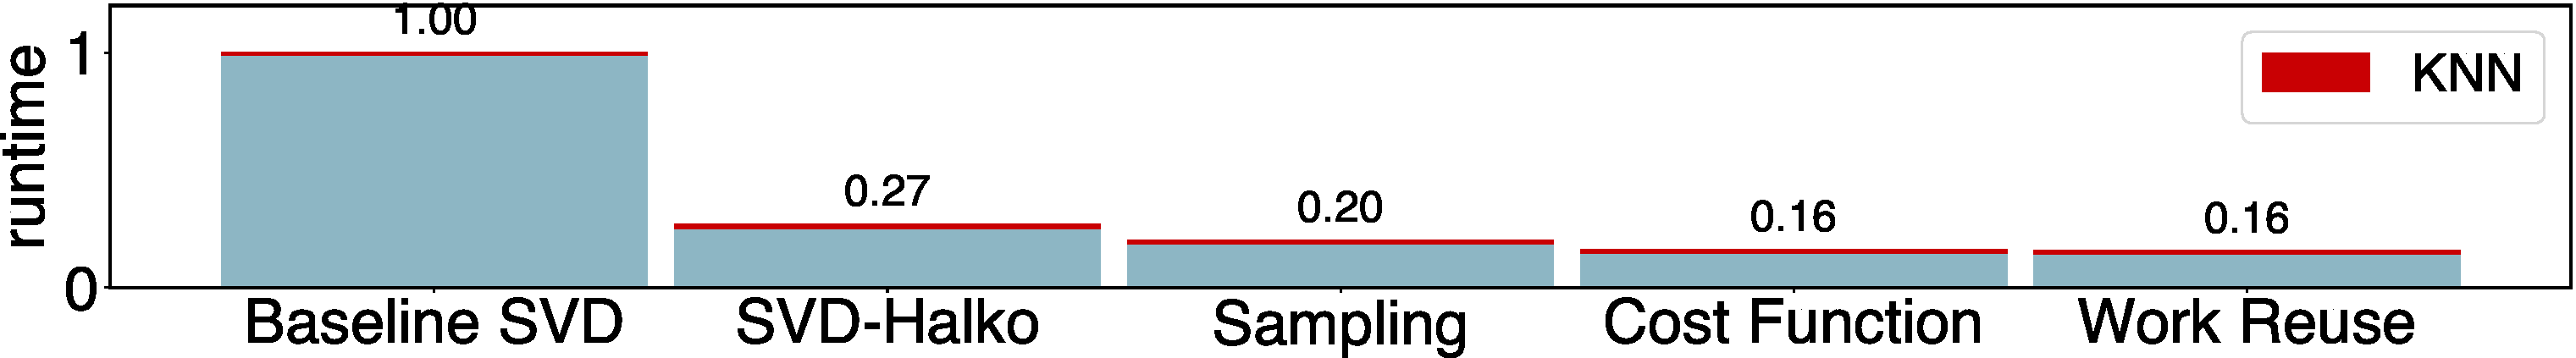
\includegraphics[width=\linewidth]{figs/yoga.pdf} 
     \caption[]{yoga}
     \end{figure} 
     

 \begin{figure}[H]
     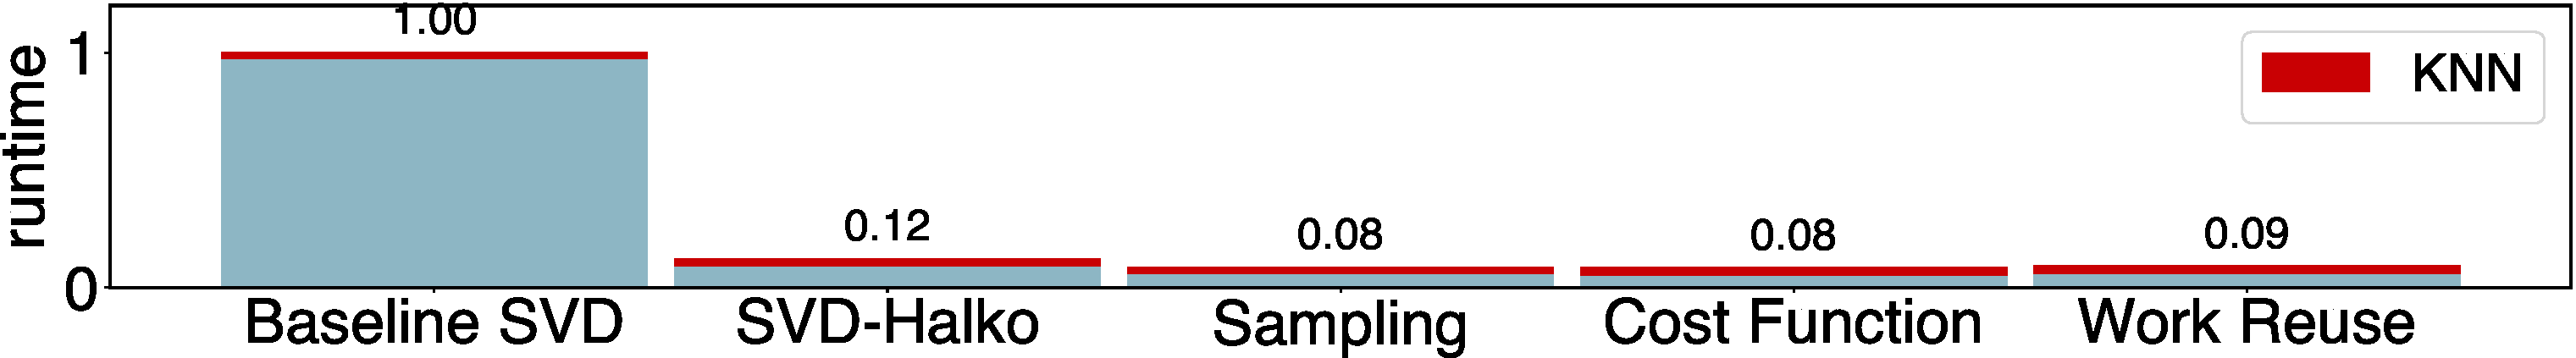
\includegraphics[width=\linewidth]{figs/uWaveGestureLibrary_Y.pdf} 
     \caption[]{uWaveGestureLibrary Y}
     \end{figure} 
     

 \begin{figure}[H] 
     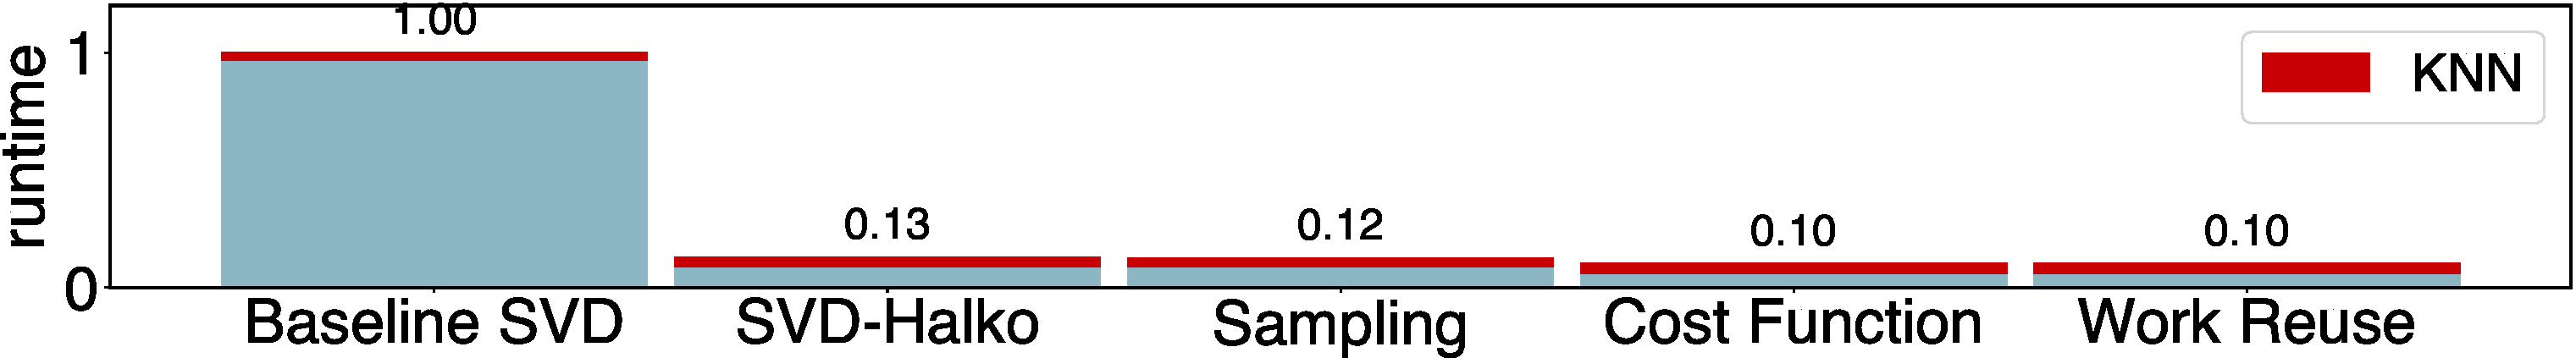
\includegraphics[width=\linewidth]{figs/uWaveGestureLibrary_X.pdf} 
     \caption[]{uWaveGestureLibrary X}
     \end{figure} 
     

 \begin{figure}[H] 
     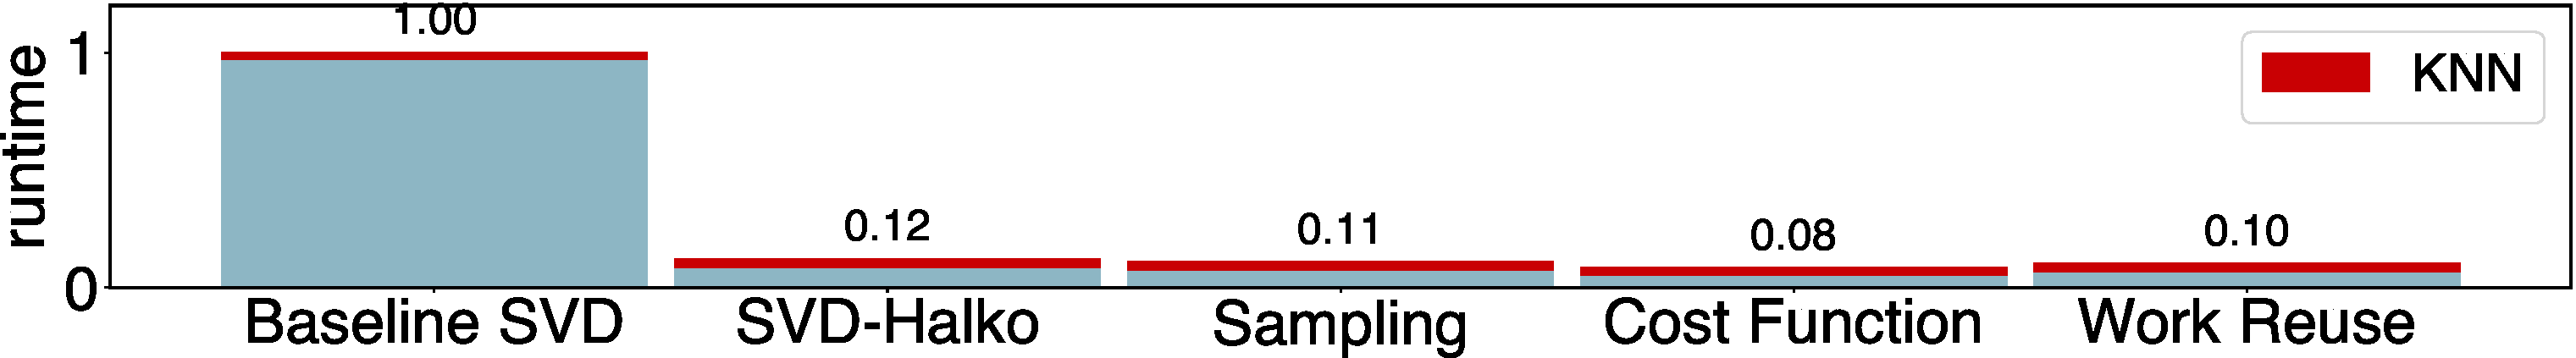
\includegraphics[width=\linewidth]{figs/uWaveGestureLibrary_Z.pdf} 
     \caption[]{uWaveGestureLibrary Z}
     \end{figure} 
     

 \begin{figure}[H] 
     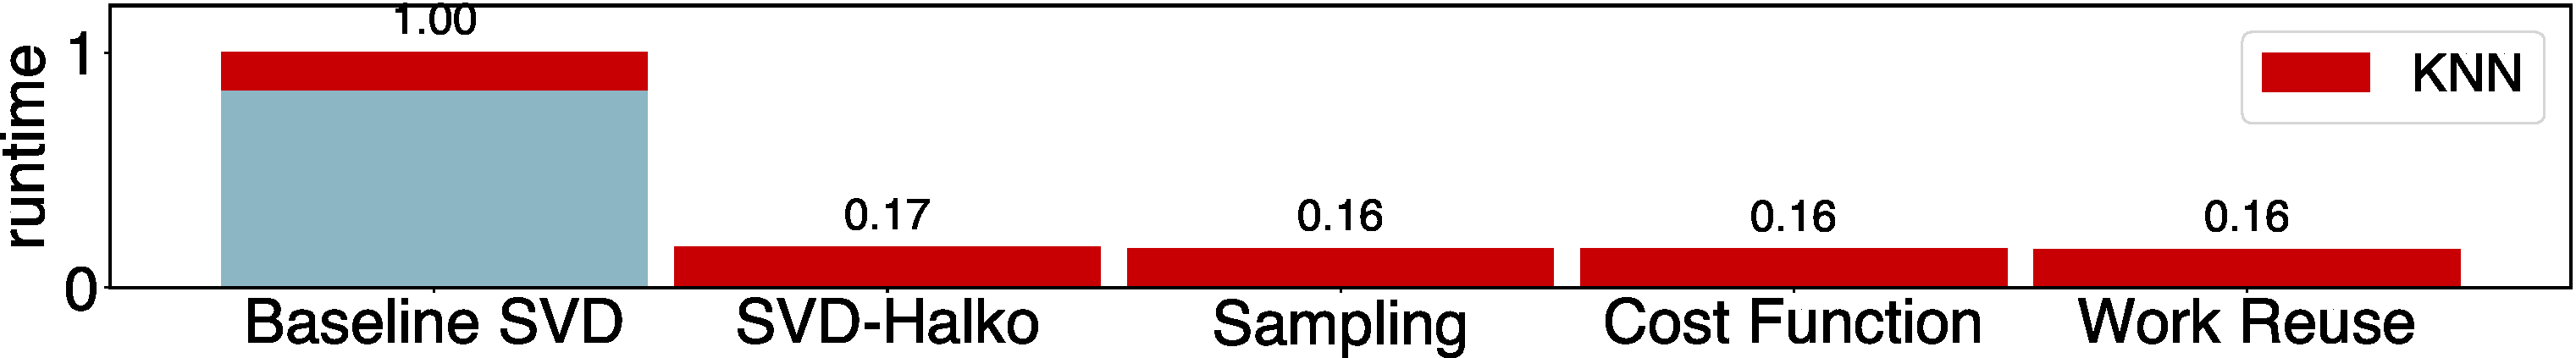
\includegraphics[width=\linewidth]{figs/ElectricDevices.pdf} 
     \caption[]{ElectricDevices}
     \end{figure} 
 
     

 \begin{figure}[H] 
     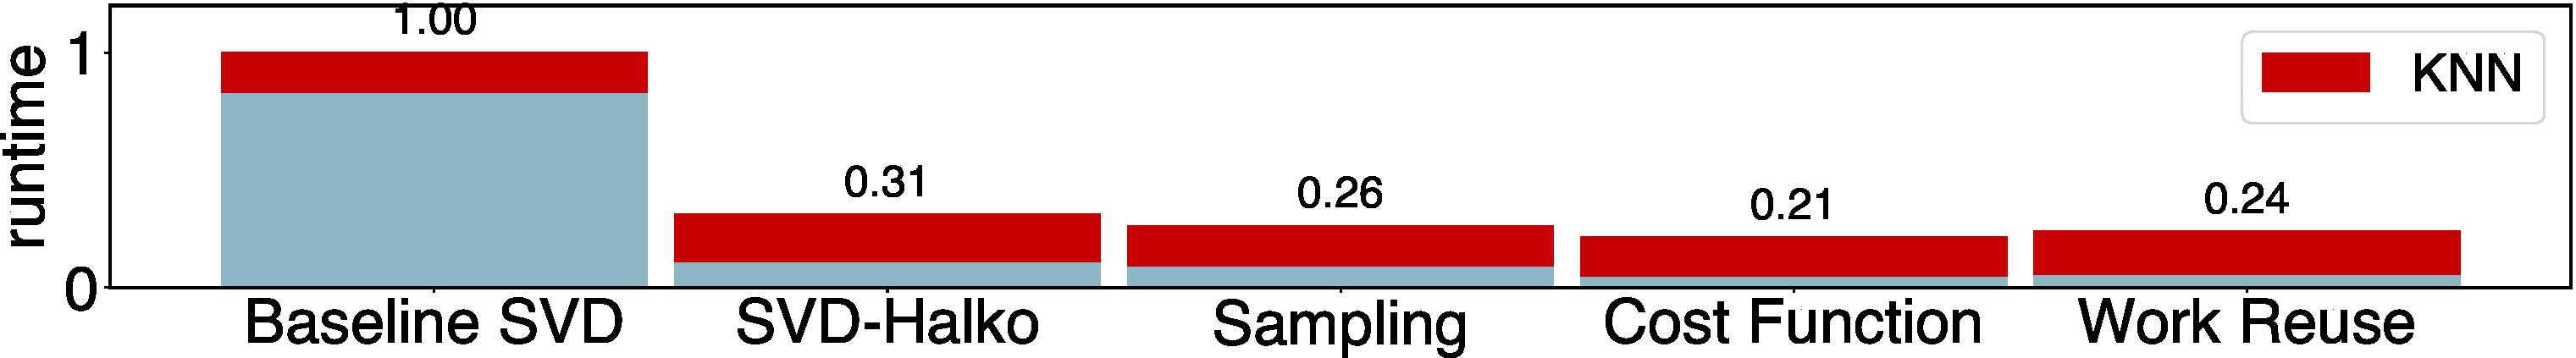
\includegraphics[width=\linewidth]{figs/FordB.pdf} 
     \caption[]{FordB}
     \end{figure} 
     

 \begin{figure}[H] 
     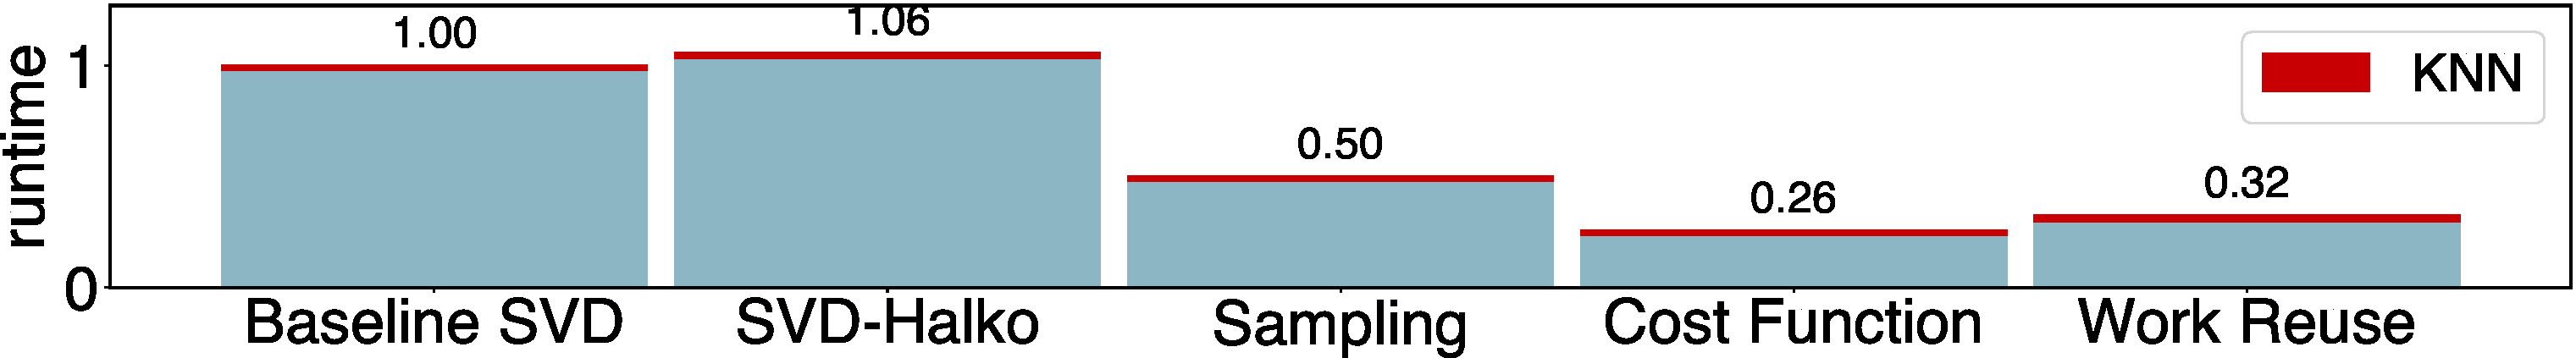
\includegraphics[width=\linewidth]{figs/MALLAT.pdf} 
     \caption[]{MALLAT}
     \end{figure} 
     

 \begin{figure}[H] 
     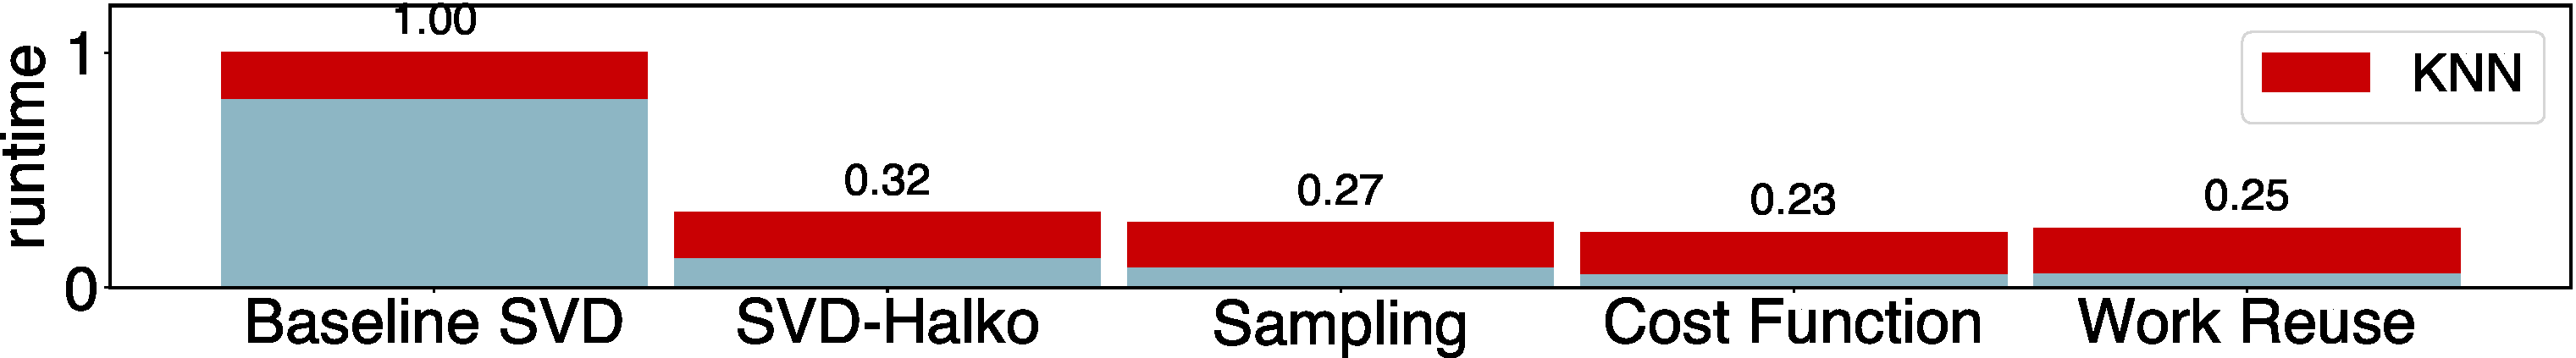
\includegraphics[width=\linewidth]{figs/FordA.pdf} 
     \caption[]{FordA}
     \end{figure} 
     

 \begin{figure}[H] 
     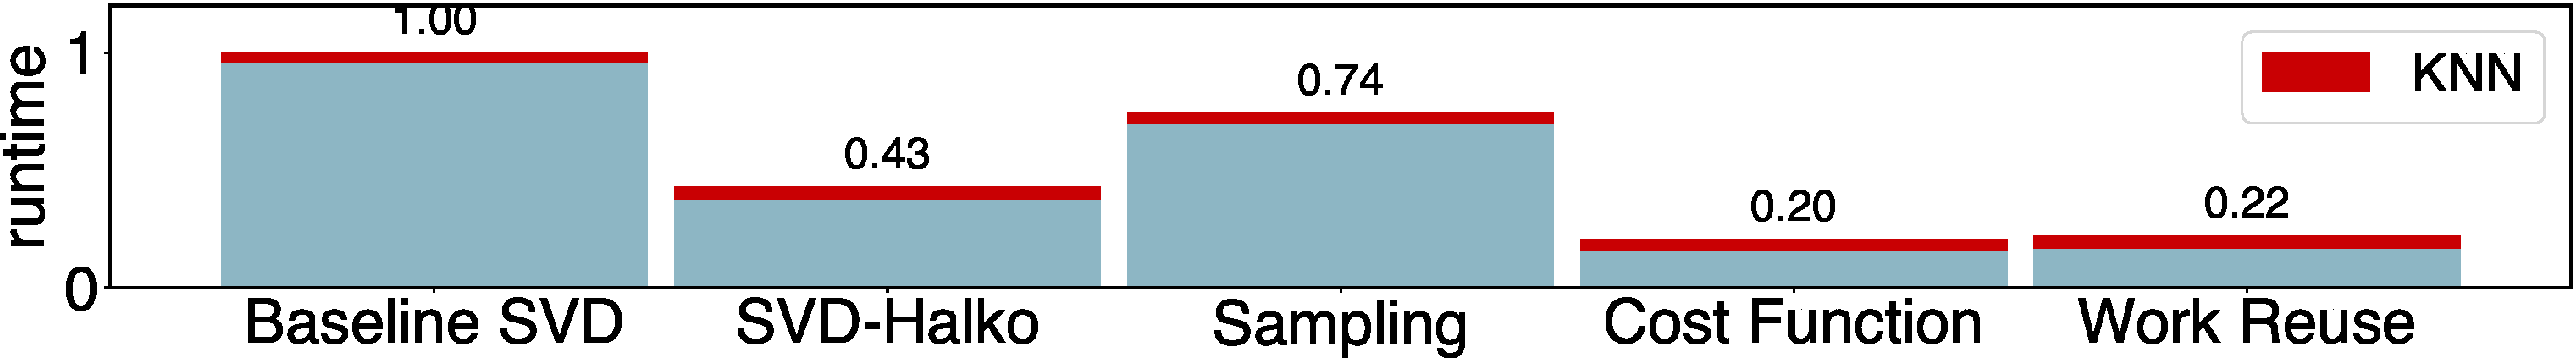
\includegraphics[width=\linewidth]{figs/NonInvasiveFatalECG_Thorax1.pdf} 
     \caption[]{NonInvasiveFatalECG Thorax1}
     \end{figure} 
     

 \begin{figure}[H] 
     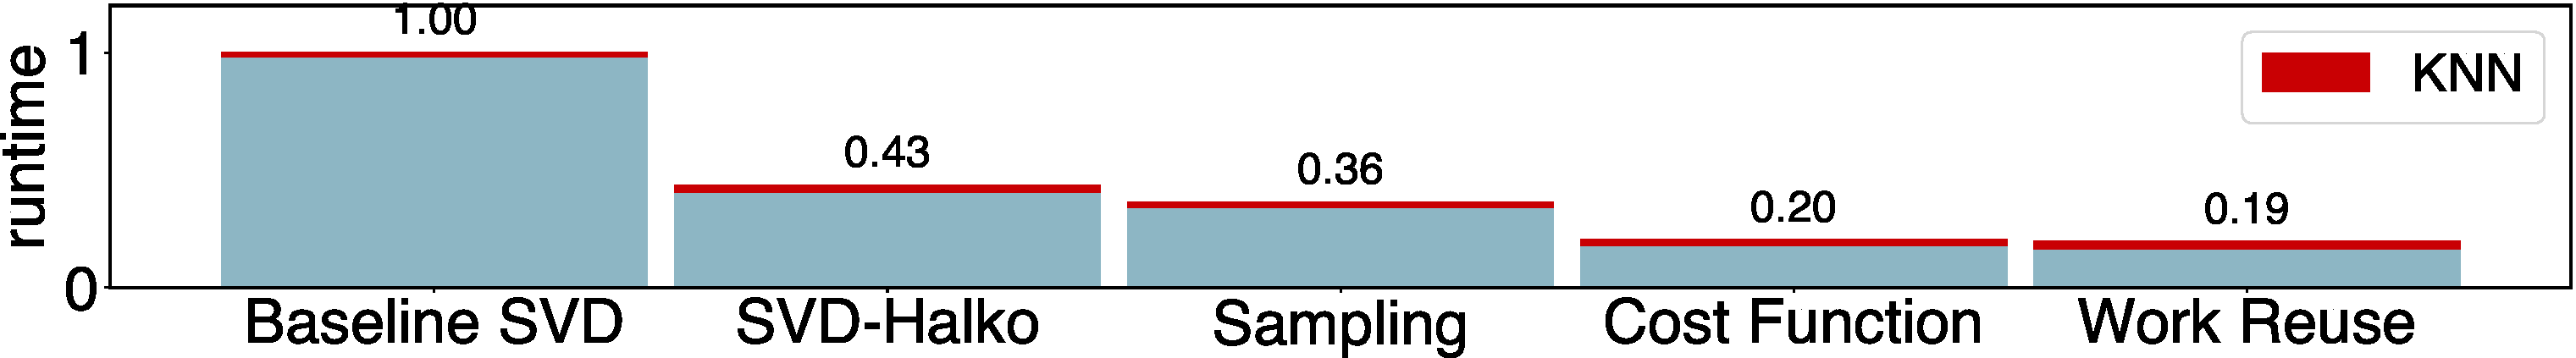
\includegraphics[width=\linewidth]{figs/NonInvasiveFatalECG_Thorax2.pdf} 
     \caption[]{NonInvasiveFatalECG Thorax2}
     \end{figure} 
     

 \begin{figure}[H] 
     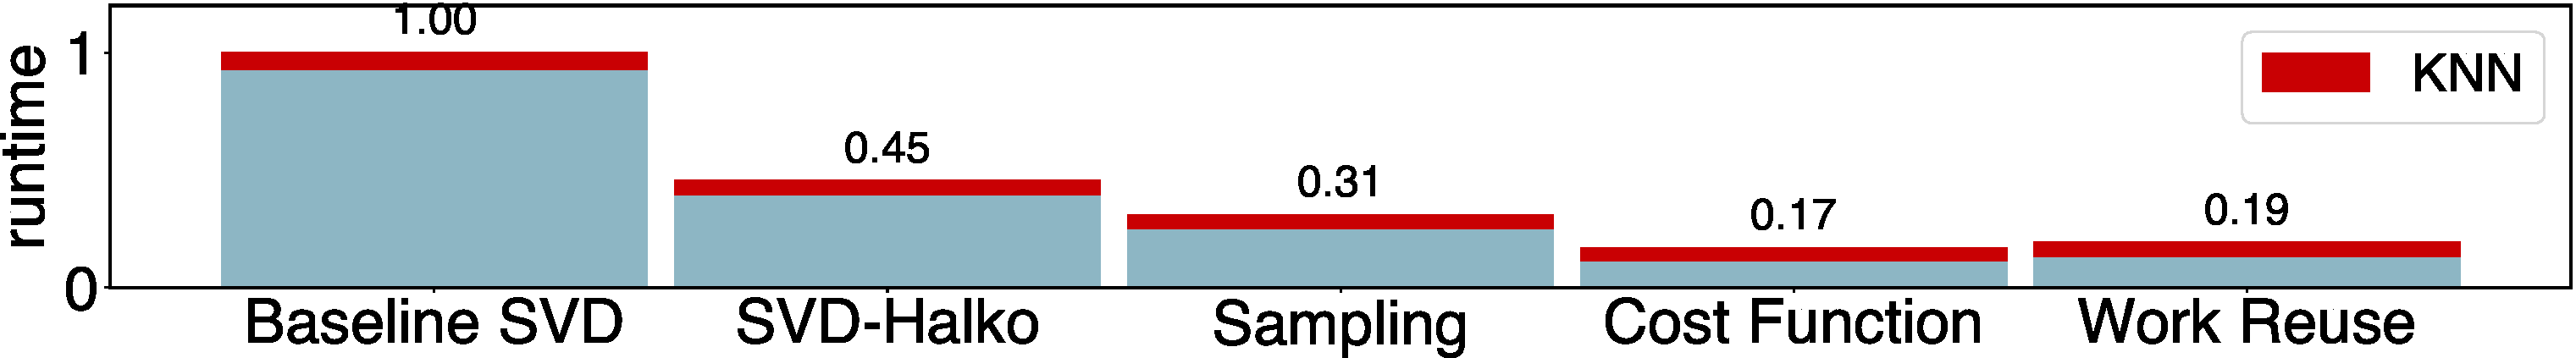
\includegraphics[width=\linewidth]{figs/UWaveGestureLibraryAll.pdf} 
     \caption[]{UWaveGestureLibraryAll}
     \end{figure} 
     

 \begin{figure}[H] 
      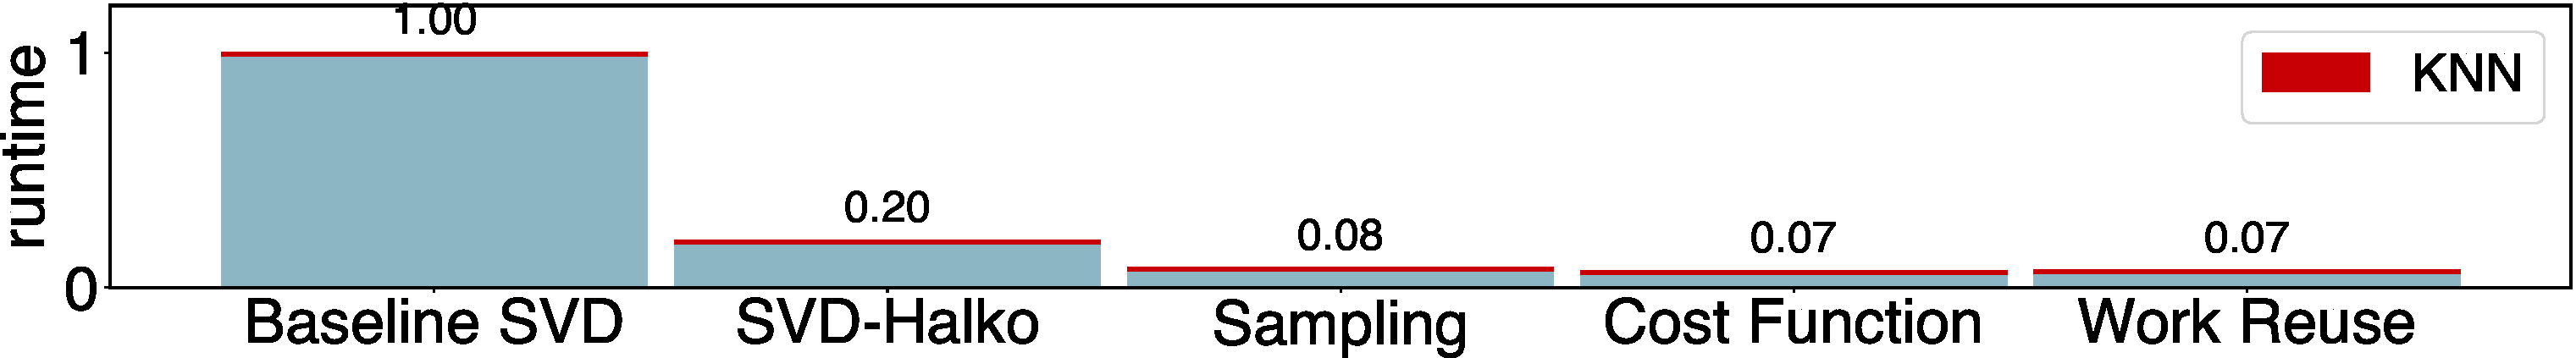
\includegraphics[width=\linewidth]{figs/StarLightCurves.pdf} 
     \caption[]{StarLightCurves}
     \end{figure} 
\end{comment}



%\input{endendplots}
